%%%%%%%%%%%%%%%%%%%%%%%%%%%%%%%%%%%%%%%%%
% Beamer Presentation
% LaTeX Template
% Version 1.0 (10/11/12)
%
% This template has been downloaded from:
% http://www.LaTeXTemplates.com
%
% License:
% CC BY-NC-SA 3.0 (http://creativecommons.org/licenses/by-nc-sa/3.0/)
%
%%%%%%%%%%%%%%%%%%%%%%%%%%%%%%%%%%%%%%%%%

%----------------------------------------------------------------------------------------
%	PACKAGES AND THEMES
%----------------------------------------------------------------------------------------

\documentclass{beamer}

\definecolor{sblue}  {RGB}{20,90,170}
\definecolor{lgreen} {RGB}{10,220,50}
\definecolor{lred}   {RGB}{220,0,0}

\newcommand{\E}{\mathbb{E}}
\newcommand{\R}{\mathbb{R}}
\newcommand{\N}{\mathbb{N}}
\newcommand{\I}{\mathbb{I}}
\newcommand{\tpsi}{\tilde{\psi}}
\newcommand{\hpsi}{\hat{\psi}}
\newcommand{\tPsi}{\tilde{\Psi}}
\newcommand\given[1][]{\:#1\vert\:}
\newcommand{\var}{\mathrm{\mathbb{V}ar}}
\newcommand{\cov}{\mathrm{\mathbb{C}ov}}
\newcommand{\corr}{\mathrm{corr}}
\newcommand{\vect}[1]{\boldsymbol{#1}}
\newcommand{\vectg}[1]{\boldsymbol{#1}}
\newcommand{\bd}[1]{\boldsymbol{#1}}
\newcommand{\idx}[3][]{{#2}^{(#3)}_{#1}}
\newcommand{\bidx}[3][]{\bd{#2}^{(#3)}_{#1}}
\newcommand{\aidx}[3][]{#2^{\langle#3\rangle}_{#1}}
\newcommand{\col}[1]{\textcolor{lred}{#1}}

\usepackage{tikz}
\usepackage{graphicx}
\graphicspath{{./img/}}


\mode<presentation> {

% The Beamer class comes with a number of default slide themes
% which change the colors and layouts of slides. Below this is a list
% of all the themes, uncomment each in turn to see what they look like.

%\usetheme{default}
%\usetheme{AnnArbor}
%\usetheme{Antibes}
%\usetheme{Bergen}
%\usetheme{Berkeley}
%\usetheme{Berlin}
%\usetheme{Boadilla}
%\usetheme{CambridgeUS}
%\usetheme{Copenhagen}
%\usetheme{Darmstadt}
%\usetheme{Dresden}
%\usetheme{Frankfurt}
%\usetheme{Goettingen}
%\usetheme{Hannover}
%\usetheme{Ilmenau}
%\usetheme{JuanLesPins}
%\usetheme{Luebeck}
\usetheme{Madrid}
%\usetheme{Malmoe}
%\usetheme{Marburg}
%\usetheme{Montpellier}
%\usetheme{PaloAlto}
%\usetheme{Pittsburgh}
%\usetheme{Rochester}
%\usetheme{Singapore}
%\usetheme{Szeged}
%\usetheme{Warsaw}

% As well as themes, the Beamer class has a number of color themes
% for any slide theme. Uncomment each of these in turn to see how it
% changes the colors of your current slide theme.

%\usecolortheme{albatross}
%\usecolortheme{beaver}
%\usecolortheme{beetle}
%\usecolortheme{crane}
%\usecolortheme{dolphin}
%\usecolortheme{dove}
%\usecolortheme{fly}
%\usecolortheme{lily}
%\usecolortheme{orchid}
%\usecolortheme{rose}
%\usecolortheme{seagull}
%\usecolortheme{seahorse}
%\usecolortheme{whale}
%\usecolortheme{wolverine}

%\setbeamertemplate{footline} % To remove the footer line in all slides uncomment this line
 %\setbeamertemplate{footline}[page number] % To replace the footer line in all slides with a simple slide count uncomment this line

\setbeamertemplate{navigation symbols}{} % To remove the navigation symbols from the bottom of all slides uncomment this line
}

\usepackage{graphicx} % Allows including images
\usepackage{booktabs} % Allows the use of \toprule, \midrule and \bottomrule in tables

%----------------------------------------------------------------------------------------
%	TITLE PAGE
%----------------------------------------------------------------------------------------

\title[AAEs for Text]{Adversarial Auto-Encoders (AAEs) and \\ Wasserstein Auto-Encoders (WAEs)}

\author[A. Lin \and M. Yu]{Alex Lin \and Melissa Yu} 
\institute[Harvard University]{Harvard University}
\date{\today}

\begin{document}

\begin{frame}
\frametitle{Overview: Adversarial Auto-Encoders for Text} 
\begin{itemize}
\item Motivation: Learning Latent Representations for Text
\begin{itemize}
\item Semi-supervised Learning
\item Text style transfer
\end{itemize}

\begin{center}
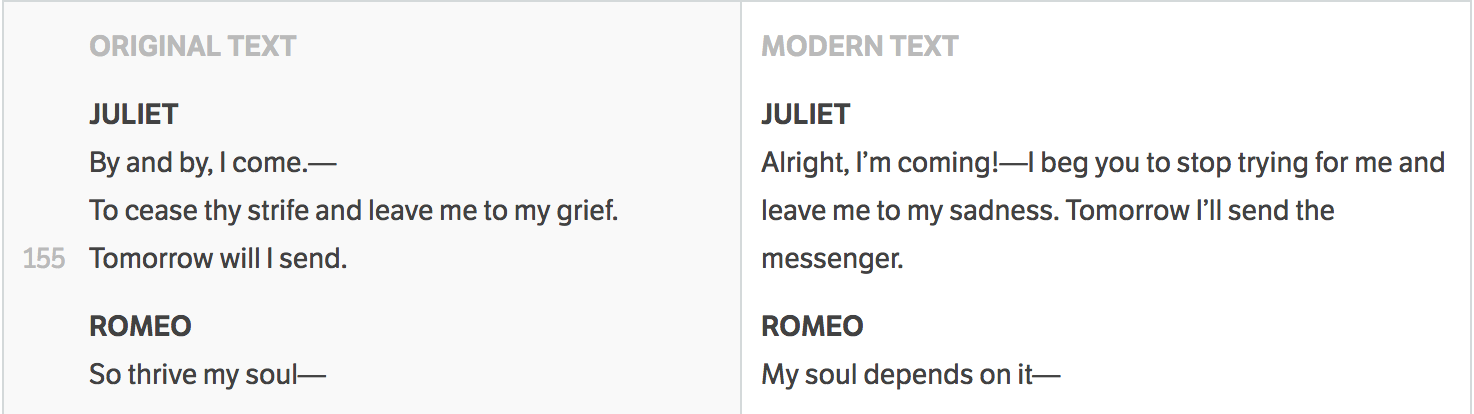
\includegraphics[scale=0.4]{shakespeare}
\end{center}

\item Several challenges
\begin{itemize}
\item VAEs reduce to prior-ignoring language models
\item GANs cannot deal with discrete observations
\item AAEs experience mode-collapse \& repeatedly generate same samples
\end{itemize}
\end{itemize}
\end{frame}

\begin{frame}
\frametitle{Adversarially Regularized Auto-Encoder (Zhao et. al, 2017)} 
\begin{itemize}
\item ARAE = discrete AAE + WGAN + learned prior
\item Improvements in semi-supervised learning
\item State-of-the-art on \emph{unaligned} text style transfer 
\end{itemize}
\begin{center}
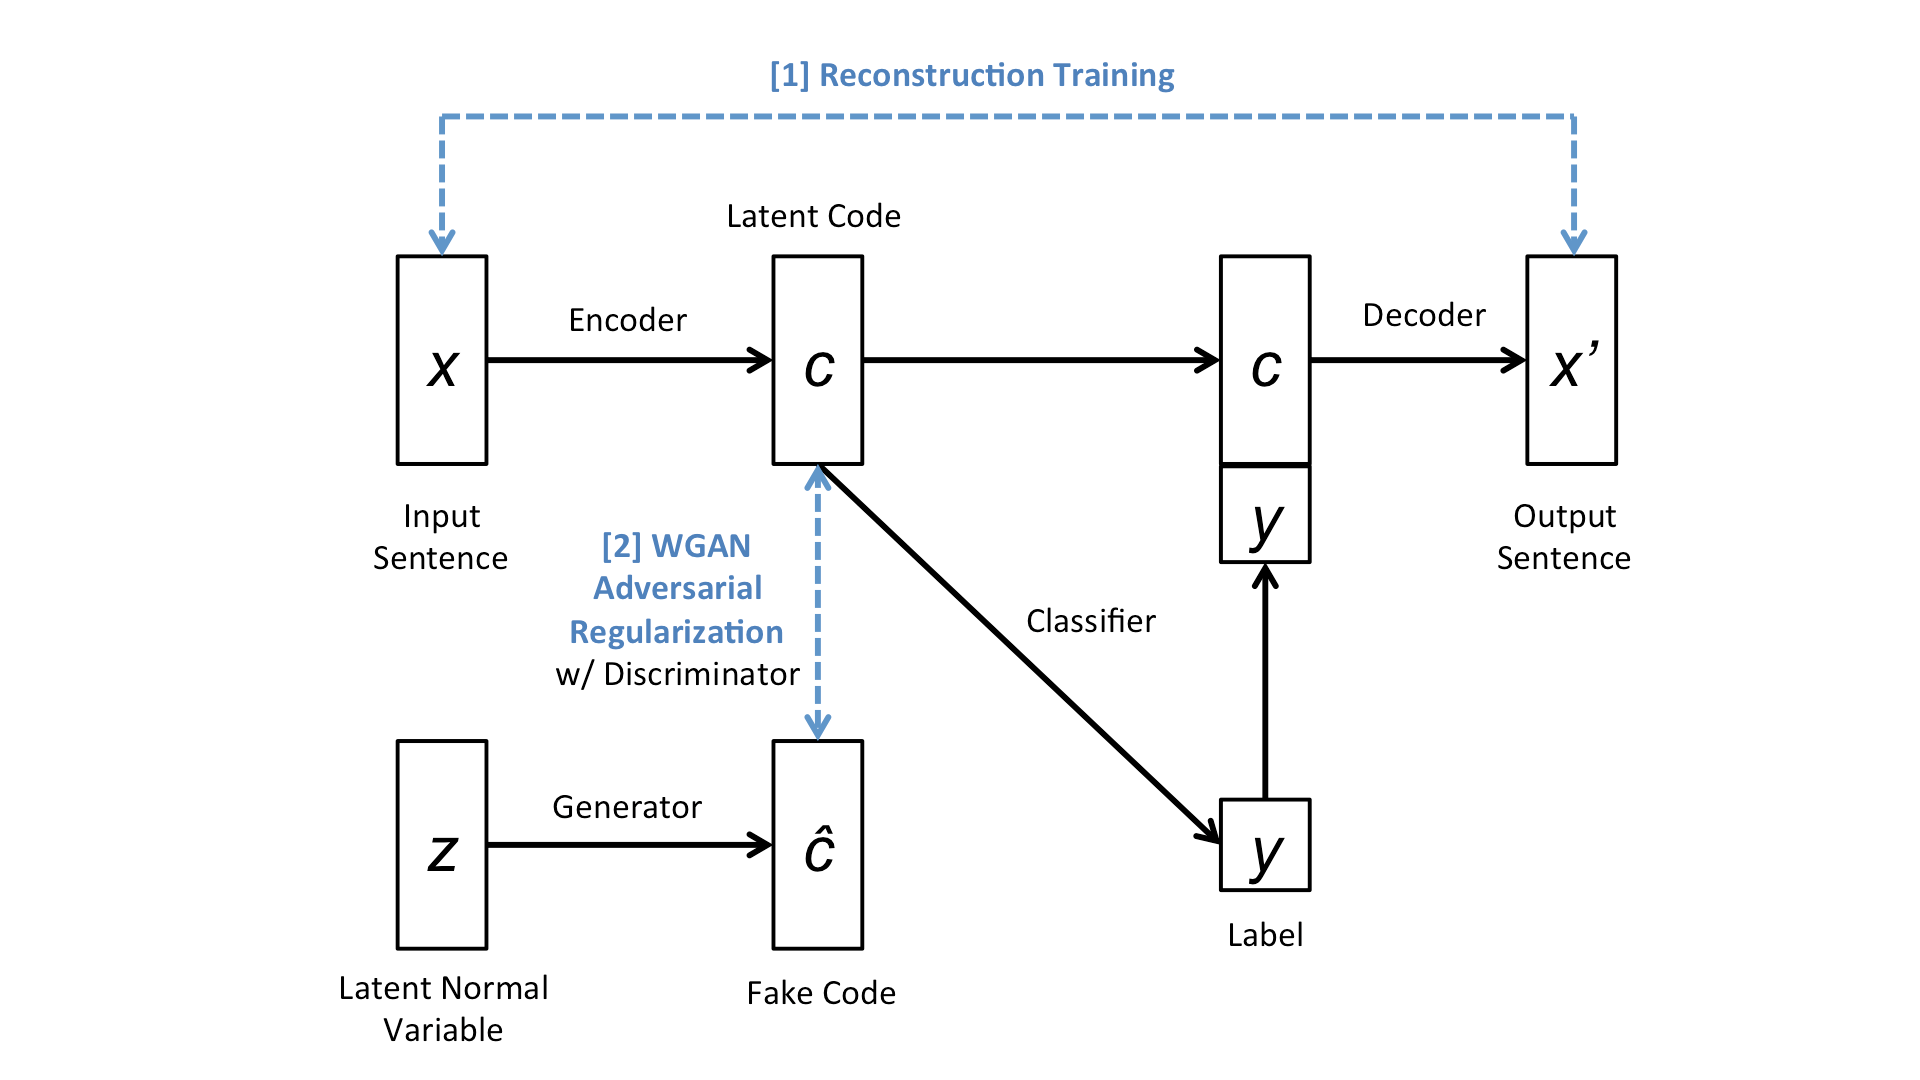
\includegraphics[scale=0.15]{arae}
\end{center}
\end{frame}

\begin{frame}
\frametitle{Next Idea: Disentangled ARAE} 
\begin{itemize}
\item Separate the \emph{label} from the \emph{code} (e.g. style) in latent space
\item Use a GAN to train the label to be categorical
\end{itemize}
\begin{center}
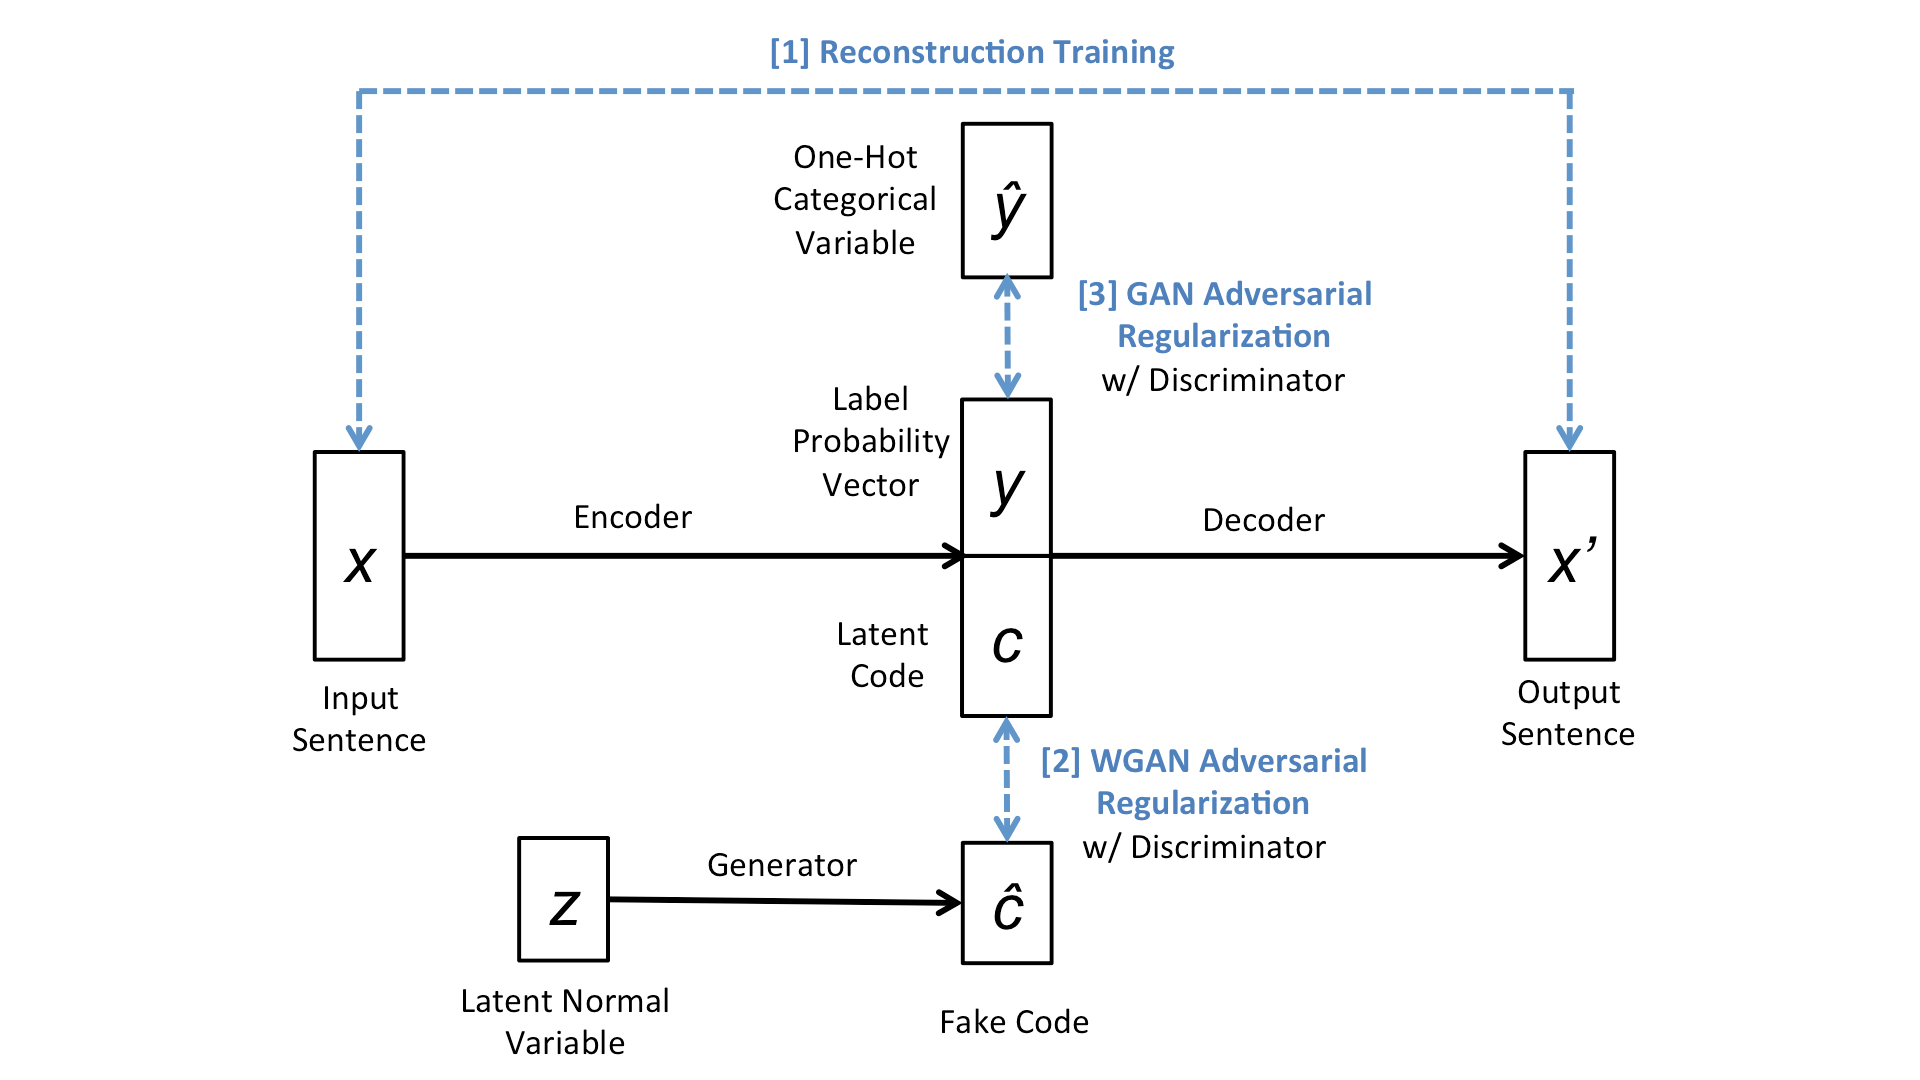
\includegraphics[scale=0.15]{our-aae}
\end{center}
\end{frame}

\end{document} 